\documentclass[12pt, oneside, a4paper, brazil]{abntex2}
% \usepackage[utf8]{inputenc}
\usepackage[brazil]{babel}
% \usepackage[T1]{fontenc}
\usepackage{fontspec}
\usepackage{setspace}
\usepackage{graphicx}
\usepackage{scalefnt}
\usepackage{float}
\usepackage[a4paper, left=3cm, right=2.5cm, top=3cm, bottom = 2.5cm]{geometry}
\usepackage{hyperref}
\usepackage{listings}
\usepackage{color}
\usepackage{titlesec}
%\usepackage[alf]{abntex2cite}
% \usepackage{times}
\usepackage[scaled]{helvet}
\usepackage{fancyhdr}
\usepackage{lmodern}


%%% Definição de variáveis. %%%
% ---
% Informações de dados para CAPA e FOLHA DE ROSTO
% ---
\titulo{Análise de desempenho de estruturas de dados para um indexador de arquivos}
\autor{Atílio Antônio Dadalto \\ Tiago da Cruz Santos}
\local{Vitória}
\data{2019}
\instituicao{%
  Universidade Federal do Espírito Santo
  \par Departamento de Informática}
\tipotrabalho{Relatório}
\preambulo{Relatório apresentado como requisito parcial para aprovação na disciplina de Programação I, pela Universidade Federal do Espírito Santo.}

\newcommand{\versao}{2.0}
\newcommand{\subtitulo}{Anteprojeto}


% Macros específicas do trabalho.
% (*) Inclua aqui termos que são utilizados muitas vezes e que demandam formatação especial.
% Os exemplos abaixo incluem i* (substituindo o asterisco por uma estrela) e Java com TM em superscript.
% Use sempre \xspace para que o LaTeX inclua espaço em branco após a macro somente quando necessário.
\newcommand{\istar}{\textit{i}$^\star$\xspace}
\newcommand{\java}{Java\texttrademark\xspace}
\newcommand{\latex}{\LaTeX\xspace}


%%% Configurações finais de aparência. %%%

% Altera o aspecto da cor azul.
\definecolor{blue}{RGB}{41,5,195}

% Informações do PDF.
\makeatletter
\hypersetup{
	pdftitle={\@title}, 
	pdfauthor={\@author},
	pdfsubject={\imprimirpreambulo},
	pdfcreator={LaTeX with abnTeX2},
	pdfkeywords={abnt}{latex}{abntex}{abntex2}{trabalho acadêmico}, 
	colorlinks=true,				% Colore os links (ao invés de usar caixas).
	linkcolor=blue,					% Cor dos links.
	citecolor=blue,					% Cor dos links na bibliografia.
	filecolor=magenta,				% Cor dos links de arquivo.
	urlcolor=blue,					% Cor das URLs.
	bookmarksdepth=4
}
\makeatother

% Espaçamentos entre linhas e parágrafos.
\setlength{\parindent}{1.3cm}
\setlength{\parskip}{0.2cm}



%%% Páginas iniciais do documento: capa, folha de rosto, ficha, resumo, tabelas, etc. %%%

% Compila o índice. <--- Desnecessário em Plano de Estudo.
%\makeindex

% Inicia o documento.
\begin{document}

% Retira espaço extra obsoleto entre as frases.
\frenchspacing


% Brasão da instituição.
\begin{figure}[h]
  \centering
  
\includegraphics[scale=0.055]{figuras/brasao}
\end{figure} 

% Capa do trabalho.
\imprimircapa
\imprimirfolhaderosto

% Lista de silgas.
% (*) Indicar as siglas utilizadas no trabalho como no exemplo abaixo.
%\begin{siglas}
    %\item [UML] Linguagem de Modelagem Unificada, do inglês \textit{Unified Modeling Language}
%\end{siglas}

% Índice de capítulos.
% \tableofcontents*


%%% Início da parte de conteúdo do documento. %%%

% Marca o início dos elementos textuais.
\clearpage
\textual

% Inclusão dos capítulos.
% (*) Para facilitar a organização, os capítulos foram divididos em arquivo separados e colocados dentro da.
% pasta capitulos/. Caso o aluno prefira trabalhar com um só arquivo, basta substituir os comandos \input 
% pelos conteúdos dos arquivos que estão sendo incluídos, excluindo a pasta capitulos/ em seguida.

\chapter*{Introdução}\label{cap-introducao} % Basicamente finalizado

Este trabalho tem por objetivo documentar a estruturação de um projeto de auxílio à tomada de decisões dado um cenário hipotético de um ambiente acidentado. Neste, dados serão extraídos por robôs-célula que investigam o local, que serão processados de forma a aprimorar a atividade de resgate das vítimas que se encontram no ambiente. O plano de testes, presentes no Capítulo~\ref{cap-planejamento-implementacao}, relata a confiabilidade das funções desenvolvidas.

As referências para os métodos de testes, bem como paradigmas aplicativo e recursivo, que serão implementados podem ser encontrados nas notas de aula utilizadas pela disciplina encontradas na página desta em maio de 2019.

Além do plano de testes, no Capítulo~\ref{cap-planejamento-implementacao} também abordamos a forma como planejamos a resolução de cada problema apresentado pelo trabalho, assim como a implementação, de forma geral, das funções mais complexas. Em seguida, o Capítulo~\ref{cap-analise-resultados} realiza uma avaliação da solução final e discorre acerca dos resultados obtidos, também pontuando comentários adicionais.
\chapter{Planejamento e implementação}\label{cap-planejamento-implementacao}

\section{Problema A}\label{problemaA}
\begin{enumerate}[label=\textbf{\alph*)},series=problemas]
\item Calcular a distância percorrida por um determinado robô ao longo do processo de resgate das vítimas. Considere que a distância total percorrida deve ser calculada como a soma de todas as distâncias entre os pontos de passagem do robô.
\end{enumerate}

\noindent \textbf{COMPREENSÃO DO PROBLEMA E PLANEJAMENTO}: deve-se extrair a tupla de um robô da lista de entrada, de acordo com o identificador dado. Em seguida, calcular a distância total que o robô percorreu e retornar esse valor.

Sendo assim, podemos criar as seguintes funções para solucionar o problema:
\begin{enumerate}
    \item Função para somar todos os elementos de uma lista
    \item Função para cálculo de distância no plano cartesiano
    \item Função para extrair uma tupla de uma lista dado um elemento identificador da tupla
    \item Função para calcular a distância entre os pontos percorridos pelo robô, por ordem de instante\label{itemDistInstante}
    \item Função para ordenar lista por instante (talvez não precise disso, precisamos ver o exemplo de entrada)
\end{enumerate}

As duas primeiras são triviais e foram implementadas diversas vezes durante o curso. Na terceira, utilizamos [...] para retornar a tupla que desejávamos. Para o item \ref{itemDistInstante}, [...].

\section{Problema B}\label{problemaB}
\begin{enumerate}[label=\textbf{\alph*)},resume*=problemas]
\item Determine qual dos robôs apresenta o seu último ponto de passagem no terreno de busca que possui a maior distância em relação à origem. Exiba o caminho percorrido pelo robô e o tempo total do percurso;
\end{enumerate}


% # - Extrair, da lista de entrada, o último ponto de passagem de todos os robôs
% # - Determinar qual robô possui ponto mais longe da origem
% # - Imprimir caminho percorrido pelo robô, determinar tempo do percurso

\section{}
\chapter{Análise  e resultados}
\label{sec-metodo}

\chapter{Conclusão}\label{cap-conclusao}

Descrever a metodologia dos testes, como variou o tamanho dos arquivos, quantos arquivos foram utilizados, descrição do computador em que foram feitos os testes.

\section{Resultados}

Analisar os tamanhos dos arquivos compactados a partir dos experimentos realizados. Utilizar tabelas e gráficos para ilustrar o desempenho da sua implementação.

Exemplo de utilização de tabelas.  A Tabela ~\ref{tab:cronograma-1} apresenta um cronograma de execução de um PG fictício.


\begin{table}[htb]
	\centering
	\caption{Cronograma de Atividades do primeiro semestre.}
	\label{tab:cronograma-1}
	\resizebox{\columnwidth}{!}{
		\begin{tabular}{c|c|c|c|c|c|c}
			Atividade & Janeiro/99 & Fevereiro/99  & Março/99  & Abril/99 & Maio/99 & Junho/99\\ \hline
			1&     X      &  	  X   	       &  	X	  	   & 		X	&     X   &      X    \\ \hline
			2&            &  	   	     	   &  	  X  	   & 		X	&         &           \\ \hline
			3&            &  		           &  	  X 	   & 		X   &   X     &     X      \\ \hline
			4&            &  			       &  			   & 	        &         &     X      \\ \hline
			5&            &  			       &  			   & 	        &    X    &   X       \\ \hline
			6&            &  			       &  			   & 	        &         &           \\ \hline
			7&            &  			       &  			   & 	        &         &           \\ \hline
		\end{tabular}
	}
\end{table}


A Figura \ref{fig:graf} exemplifica o uso de uma figura gráfica no texto.


   \begin{figure}[!htb]
    \centering
   	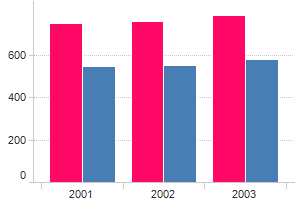
\includegraphics[scale=0.90]{figuras/graf-exemplo.png}
   	\caption{Exemplo de inserção de figura}
   	\label{fig:graf}
   \end{figure}


Discutir as conclusões e limitações do seu trabalho.

\chapter{Conclusão}
\label{sec-conclusao}


Discutir as conclusões e limitações do seu trabalho.



% Finaliza a parte no bookmark do PDF para que se inicie o bookmark na raiz e adiciona espaço de parte no sumário.
\phantompart

% Marca o fim dos elementos textuais.
\postextual

% Referências bibliográficas
\clearpage
\bibliography{bibliografia}

% Fim do documento.
\end{document}
